\documentclass[a4paper,11pt]{article}

\usepackage{mlsubmit}

\begin{document}

\initmlsubmision{2}                              					% assignment number
								{Raktim Mitra}      						           		% your name
								{150562}																		% your roll number

\begin{mlsolution}


%\begin{figure}[th]%
%\centering
%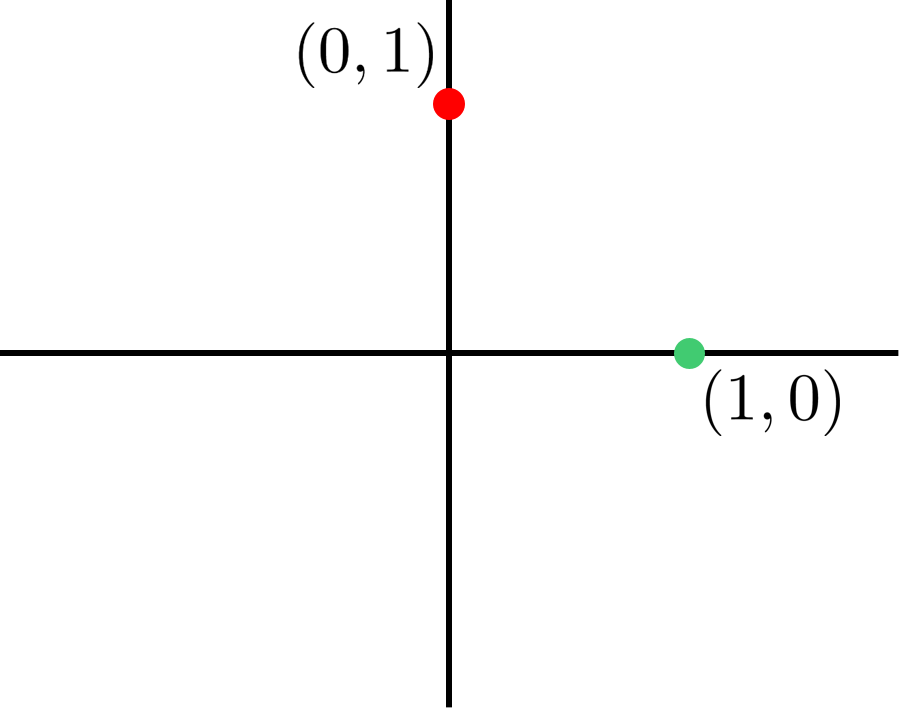
\includegraphics[width=0.3\columnwidth]{proto_blank.png}%
%\hfill
%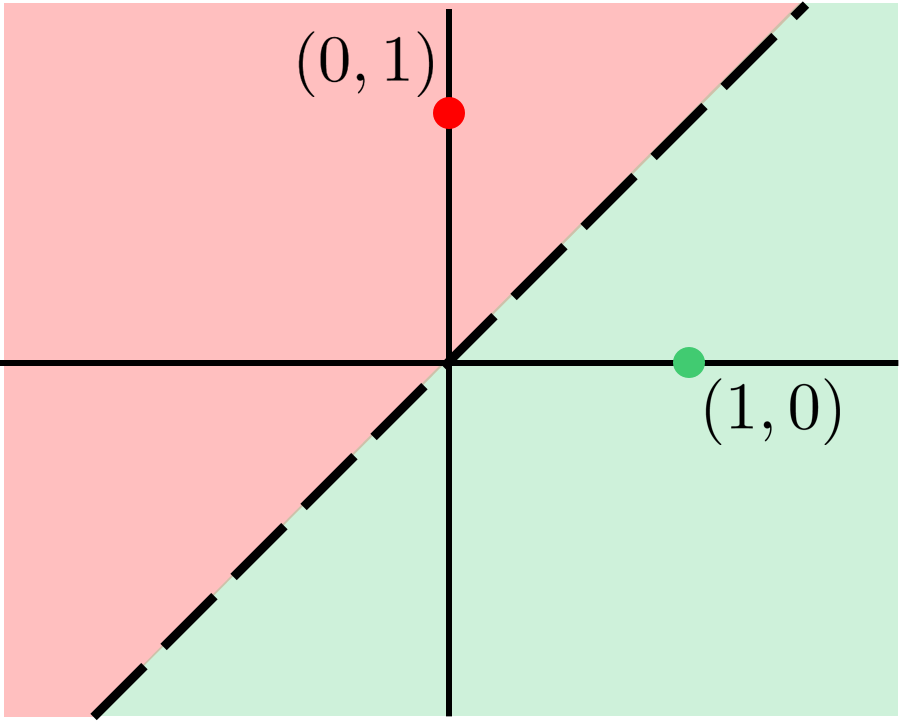
\includegraphics[width=0.3\columnwidth]{proto_euclid_sample.png}%
%\caption{Learning with Prototypes: the figure on the left shows the two prototypes. The figure on the right shows what the decision boundary if the distance measure used is $d(\vz^1,\vz^2) = \norm{\vz^1-\vz^2}_2$, for any two points $\vz^1,\vz^2 \in \bR^2$. The decision boundary in this case is the line $y = x$.}%
%\label{fig:proto}%
%\end{figure}
\subsection*{Part 1:} Row number 4 and 6 has exactly same attributes except the name and one is \textbf{Yes} while other one is \textbf{No}. That means the `Name' field will be required to separate them. Hence, that field will be useful. Same applies for 6 and 14.
\subsection*{Part 2:}
If we do not consider the \textbf{Name} attribute then it is not possible to classify the data no matter how complicated the algorithm is, because as said earlier there are pairs of rows for which all attributes are same except name but they belong to different classes.


If we consider the name attribute then it is posssible to perfectly classify the  data since no two names are same. Although \textbf{Name } is very less informative as a decision node, but to perfectly classify it is needed. 

\subsection*{Part 3:}

From the ID3 algorithm :
Information gain by choosing an attribute is calculated as:
\begin{equation}
		Gain(S,A) = Entropy(S) - \Sigma_i\frac{|S_i|}{|S|}Entropy(S_i)
\end{equation}	
		where $|S_i|$ is set of elements of S with same value of Attribute A.
Entropy of S(5 Yes, 10 No):
\begin{equation}
Entropy(S) = -\frac{5}{15}log\frac{5}{15} - \frac{10}{15}log\frac{10}{15} \\
	= 0.9183
\end{equation}
Now, values of entropy : \\
We have used $lim_{x \rightarrow 0} xlog(x) = 0$
\begin{align*}
  Entropy(S_{size=small}) &= 0.6500 \\
  Entropy(S_{size=medium}) &= 0.9710 \\
  Entropy(S_{size=large}) &= 1.0 \\
  Entropy(S_{likearea=yes}) &= 1.0 \\
  Entropy(S_{likearea=no}) &= 0.8454 \\
  Entropy(S_{workload=light}) &= 0.8113 \\
  Entropy(S_{workload=average}) &= 1.0 \\
  Entropy(S_{workload=heavy}) &= 0.7219 \\
  Entropy(S_{meetings=0-1}) &= 0.9710 \\
  Entropy(S_{meetings=2-3}) &= 0.0 \\
  Entropy(S_{meetings>3}) &= 0.0 \\  
\end{align*}
Gain calculation for root node:
\begin{align*}
  Gain(S,size) &= 0.0680 \\
  Gain(S,like) &= 0.0317 \\
  Gain(S,workload) &= 0.0613 \\
  Gain(S,meetings) &= 0.2710 \\
\end{align*}
Conditioning on \textbf{number of meetings} attribute gives maximum gain, so root will use this attribute to separate.
\begin{align*}
  Gain(S_{0-1,workload}) &= 0.41 \\
  Gain(S_{0-1,research area}) &= 0.0587 \\
  Gain(S_{0-1},size) &= 0.085 \\
\end{align*}
Hence the 0-1 branch from root will use \textbf{workload} as next attribute to branch upon.
\begin{figure}[th]%
\centering

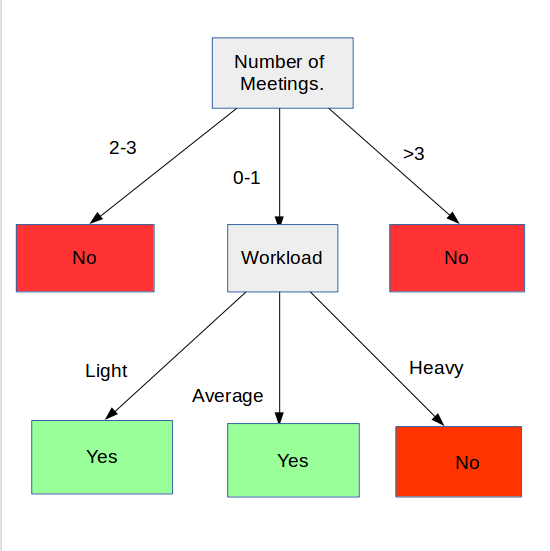
\includegraphics[width=0.6\columnwidth]{q4/dt.png}%

\caption{Decision Tree}
\label{fig:proto}%
\end{figure}

Number of Meetings 2-3 and NUmber of Meetings >3 results into two pure leaf nodes with  No labels.

From 0-1 path at workload node 3 branches are generated from the node using workload as attribute. The average node becomes pure leaf node. The light node has a tie with  1 Yes and 1 No. Arbitrarily assigning it a Yes leaf node. The Heavy node has a majority of No, so making it a No leaf node.
\end{mlsolution}

\begin{mlsolution}
\subsection*{Part 1:}
We want to model $\mathbb{P}[b^i | \mathbf{x^i,\Theta}]$. We can write it using conditional probability, summed over all possible combinations , as follows:
\begin{align*}
\mathbb{P}[b^i | \mathbf{x^i,\Theta}] = \sum_{j=1}^{2^L}\mathbb{P}[b^i| S^j,\mathbf{x^i,\Theta}].\mathbb{P}[S^j|\mathbf{x^i,\Theta}]
\end{align*} 

Probability $\mathbb{P}[b^i | S^j,\mathbf{x^i,\Theta}]$ is modeled from $\mathcal{N}(\mu_i,\sigma^2)$ .

Now we assume the customers choice among products are independent and hence we get $\mathbb{P}[S^j|\mathbf{x^j,\Theta}] = \prod_{k=1}^{L}\mathbb{P}[S_k^j|\mathbf{x^j,\Theta}]$.

Using hint, we model $\mathbb{P}[S_k^j = 1 | \mathbf{x^j,\Theta}] = sigmoid\langle w_k,x^j\rangle$ 

Our Model $\Theta = \{\mathbf{W}={\mathbf{w}_i}\forall i\epsilon[L], \mu_i\forall i\epsilon[n],\sigma\}$

$S^i$'s are our latent variables in this problem. 
Using all these finally our model becomes:
\begin{equation}
\mathbb{P}[b^i|x^i,\Theta]= \prod_{i=1}^{n}\sum_{j=1}^{2^L}\mathbb{P}[b| S^j,\mathbf{x,\Theta}].\Big[\prod_{k=1}^{L}\mathbb{P}[S_k^j|\mathbf{x,\Theta}] \Big]
\end{equation}
\subsection{Part 2:}
	Assuming each customer is independent, we can write $\mathbb{P}[\mathbf{b | x,\Theta}]$ as products of each customer probabilities: Here \textbf{b} is a vector of $b^i$ for each customer i.
	\begin{align*}
	\mathbb{P}[\vb|\vx, \vTheta] &= \prod_{i=1}^{n} P[b^i \cond \vx^i, \vTheta]\\
	\mathbb{P}[\vb|\vx, \vTheta] &= \prod_{i=1}^{n}\sum_{j=1}^{2^L} \P{b^i|\vx^i,S^j,\vTheta} \left[\prod_{k=1}^{L} \P{S^j_k| \vx^i, \vTheta}\right]\\
	&= \prod_{i=1}^{n}\sum_{j=1}^{2^L} \cN\left(\mu_j,\sigma^2\right) \left[\prod_{k=1}^{L} \P{S^j_k| \vx^i, \vTheta}\right]	\\
	\end{align*}
Now this gives our MLE estimate of the model: $\vTheta_{MLE} = \underset{\vTheta}{\arg\max}\ P[\vb| \vX, \vTheta]$	
	\newpage
	\subsection{Part 3:\textbf{Hard Assignment Alternating Optimization:}}
	
	
		 $>$ Initialize $\vTheta^0$.\\
		 $>$Update $S^i$ $\forall i$. We do this by finding $S^i$ such that $P[S\cond \vx^i, b^i, \vTheta^t]$ is maximised.
			\begin{align*}
				S^i &=  \underset{S^i}{\arg\max}\ \mathbb{P}[S^i|\vx^i,b^i,\vTheta] \intertext{where}
				\P{S\cond\ \vx^i, b^i, \vTheta}
							&\propto P[S^i|\vx^i, \vTheta]\prod_{j=1}^{L} \P{S^i_j| \vx^i, b^i, \vTheta}\\
							&= \mathcal{N}(\mu^i, \Sigma)\prod_{j=1}^{L} \sigma(\vw_j^T\vx^i)^{S^i_j}[1 - \sigma(\vw_j^T\vx^i)]^{1 - S^i_j}
							\intertext{We set $S_j^i$ as 1 or 0 depending on whether it's probability is greater than $0.5$ or not.}
			\end{align*}
		$>$ Now we update $\vTheta^{t+1}$ using the new obtained $S^i$.
			\begin{align*}
				\vTheta^{t+1} &= \underset{\vTheta}{\arg \max } \mathbb{P}[\mathbf{b},S| X, \vTheta]\\
							&= \underset{\vTheta}{\arg \max} \prod_{i=1}^{n} \mathbb{P}[b^i \cond S^i, x^i, \vTheta]\prod_{j=1}^{L}\mathbb{P}[S^i_j\cond \vx^i, \vTheta]\\
							&= \underset{\vTheta}{\arg \max} \prod_{i=1}^{n} \left(\mathcal{N}(\mu^i, \sigma^2)
							\prod_{j=1}^{L}\sigma(\vw_j^T\vx^i)^{S_j^i}[1 - \sigma(\vw_j^T\vx^i)]^{1 - S_j^i}\right)
							\end{align*}
	It can be easily seen using first order derivative method we find:
							$\mu_i = \sum_{j|S^i_j = 1} C_j$\\
							$\sigma_i^2 =  \frac{\sum_{i=1}^{n}(x^i - \mu^i)^2}{n}$ as expected in the problem scenario.\\
										
							$>$ Repeat until Convergence.
	\subsection{Part 4:\textbf{soft Alternating optimization algorithm:}}
		$>$For $i \in [n]$ create $2^L$ copies of datapoint $x^i$.
				$x^i to \{x^{i,1}, x^{i,2},..., x^{i,2^L}\}$\\
		$>$Initialize $\vTheta^0$.Let,$\mathcal{\pi}_j = P[S^i = j | \vx^i, \vTheta]$ which is product of linear logistics desribed in part 1.
		Update weights $\gamma^{i,k,t}$ using $\vTheta^0$
				\begin{align*}
					\gamma^{i,k,t} &= P[S^i | b^i, \vx^i, \vTheta^t]\\
					&= \frac{P[S^i = k \cond \vx^i, \vTheta]\ P[b^i\cond x^i, S^i = k, \vTheta]}
					{\sum_{j=1}^{j=2^L}P[S^i = j\cond \vx^i, \vTheta]\ P[b^i\cond x^i, S^i = j, \vTheta]}\\
					&= \frac{\mathcal{\vpi}_k^t\ \mathcal{N}(\mu_i, \sigma^2)}
					{\sum_{j=1}^{j=2^L}\mathcal{\vpi}_j^t\ \mathcal{N}(\mu_i, \sigma^2)}
				\end{align*}
		$>$ Update $\vTheta^{t+1}$,
		\begin{align*}
			\vTheta^{t+1} &= \underset{\vTheta}{\arg\max}\ P[\{\vx^{i,k}\}, \{b^{i,k}\}, \{\gamma^{i,k,t}\}]
		\end{align*}
		where $P[\vx,b,\gamma\ |\vTheta] = P[x,b|\vTheta]^\gamma$.\\
		$>$ Repeat until Convergence	
	
\end{mlsolution}

\begin{mlsolution}
\subsection*{Part 1:}
\textbf{Claim:} $\xi_i \geq 0$ constraints are vacuous. \\
\textbf{Proof:} Let there is an optimal solution with some $\xi_i < 0$. now, since $\xi_i < 0 $ it follows that $1-\xi_i > 1 - 0$ i.e. $y^i\langle \mathbf{w,x^i} \rangle$ strictly greater than 1. This means we can replace negative $\xi_i$'s with 0. That will also reduce the objective funstion by an amount $\xi_i^2$. Therefore, we have a contradiction as the solution we took as optimal is not optimal.

Hence $\xi_i$ cannot be negative in an optimal solution of the problem. Hence the $\xi_i \geq 0$ conditions are vacuous. 

Now, let there is an optimal solution of the problem with out the constraints. Then we essentially get an optimal value of $\xi_i^2$ which has anyway a positive root $\xi_i$ which is greater than or equal to 0. Hence it holds. [Proved]

\subsection{Part 2:}
	$y^i\ip{\vw}{\vx^i} \geq 1 - \xi_i \implies 1 - \xi_i - y^i\ip{\vw}{\vx^i} \leq 0$
	and $\xi_i \geq 0
	\implies -\xi_i \leq 0$

% So, introduce parameters $\alpha_i$ so that the langrangian becomes:
We introduce lagrange parameters $\alpha_i$'s and $\beta_i$'s. The langrangian becomes:
% $$ L(\vw,\bc{\xi_i}, \bc{\alpha_i}) = \norm{\vw}_2^2 + \sum_{i=1}^n\xi_i^2 + \sum_{i=1}^n \alpha_i(1 - \xi_i - y^i\ip{\vw}{\vx^i}) \qquad\qquad(L1)$$
$$ L(\vw,\bc{\xi_i}, \bc{\alpha_i}, \bc{\beta_i}) = \norm{\vw}_2^2 + \sum_{i=1}^n\xi_i^2 + \sum_{i=1}^n \alpha_i(1 - \xi_i - y^i\ip{\vw}{\vx^i}) - \sum_{i=1}^{n}\beta_i\xi_i $$
					
\subsection{Part 3:}
We want to solve objective $$\underset{\vw,\bc{\xi_i}}{\arg\min}\ \underset{\alpha_i \geq 0, \beta_i \geq 0}{\arg\max}\ \ L(\vw,\bc{\xi_i}, \bc{\alpha_i}, \bc{\beta_i})$$\\
Derivative w.r.t $\vw$:

	$2\vw + 0 + \sum_{i=1}^{n} \alpha_i * (-y^i\vx^i) = 0
	\implies \vw = \frac{\sum_{i=1}^{n} \alpha_iy^i\vx^i}{2}$\\
Derivative w.r.t $\xi_i$:

	$2\xi_i - \alpha_i - \beta_i = 0
	\implies \xi_i = \frac{\alpha_i + \beta_i}{2}$

Substituting these values in Lagrangian:
\begin{align*}
	f(\bc{\alpha_i}, \bc{\beta_i}) \\
			&= \frac{1}{4}\sum_{i=1}^{n}\sum_{j=1}^{n}\alpha_i\alpha_jy^iy^j(\vx^i)^T\vx^j + \frac{1}{4}\sum_{i=1}^{n}(\alpha_i +\beta_i)^2 +
			\sum_{i=1}^n\alpha_i
			- \sum_{i=1}^n \alpha_i y^i \ip{\frac{1}{2}\sum_{j=1}^{n} \alpha_j y^j \vx^j}{\vx^i}\\
			& \qquad-\frac{1}{2}\alpha_i(\alpha_i + \beta_i) -\frac{1}{2}\beta_i(\alpha_ + \beta_i)\\
			&= \sum_{i=1}^n \alpha_i -\frac{1}{4}\sum_{i=1}^{n}\sum_{j=1}^{n}\alpha_i\alpha_jy^iy^j(\vx^i)^T\vx^j - \sum_{i=1}^n\frac{(\alpha_i + \beta_i)^2}{4}
\end{align*}


Hence: $$f(\bc{\alpha_i}, \bc{\beta_i}) = \sum_{i=1}^n \alpha_i - \sum_{i=1}^n\frac{(\alpha_i + \beta_i)^2}{4} - \frac{1}{4} \sum_{i=1}^{n}\sum_{j=1}^{n}\alpha_i\alpha_jy^iy^j(\vx^i)^T\vx^j$$ where $\alpha_i \geq 0, \beta_i \geq 0$ $ \forall i$.\\
$(\alpha_i + \beta_i)^2$, being a non-negative quantity,it follows that the dual is maximised when it becomes as small as possible. No other term in the expression has $\beta$,hence we can set it to 0($\beta_i \geq 0$). Therefore the constraint of $\xi_i \geq 0$ was clearly vacuous. \\
Hence, the Dual Problem is finally:
$$ f(\bc{\alpha_i}) = \sum_{i=1}^n \alpha_i - \sum_{i=1}^n\frac{\alpha_i^2}{4} - \frac{1}{4} \sum_{i=1}^{n}\sum_{j=1}^{n}\alpha_i\alpha_jy^iy^j(\vx^i)^T\vx^j$$ where $\alpha_i \geq 0$ $\forall i$ 
\\ \\ 
\subsection{Part 4:}

Dual problem for original SVM :
$$f(\alpha) = \sum_{i=1}^n \alpha_i - \frac{1}{2} \sum_{i=1}^{n}\sum_{j=1}^{n}\alpha_i\alpha_jy^iy^j(\vx^i)^T\vx^j$$
where $0 \leq \alpha_i \leq C$

1. In the original SVM we have an upper bound for $\alpha_i$ which is result of the constraints $\xi_i > 0$. Here we do not have that because those constraints are vacuous here.

2. Also there is an extra summation term on $\alpha_i^2$ in this problem which is not present in original problem.

\subsection*{Part 5:}
Those $\xi_i > 0$ constraints are not vacuous for the original problem. There we basically used $\xi_i$s to allow some points to lie between the expected margin of classifications. 
Removing $\xi_i \geq 0$ would then may change the solution because it would mean we  are actually allowing to points to be present further awaya from the argin of classification. Which means we may not get the highest possible margin of classification  which we get from the constraint problem except for some allowance of points to viaolate the margin. Hence we cannot remove those constraints in the original problem.
\end{mlsolution}

\begin{mlsolution}

\subsection*{Part 3:}
In the GD implementation averaged for small number of iterations "wbar" was giving slightly better objective values and for large number of iterations there was not much noticable difference. So, I kept final averaged model for my solution.

\subsection*{Part 4:}

My best step-length selection strategy was 

$eta = \frac{c}{n}\frac{1}{\sqrt{t^k} + 1}$ where I found c = 50, k = 0.9 to work best. n is number of data points, t is iteration number.
 
\subsection*{part 5:}

\begin{figure}[th]%
\centering

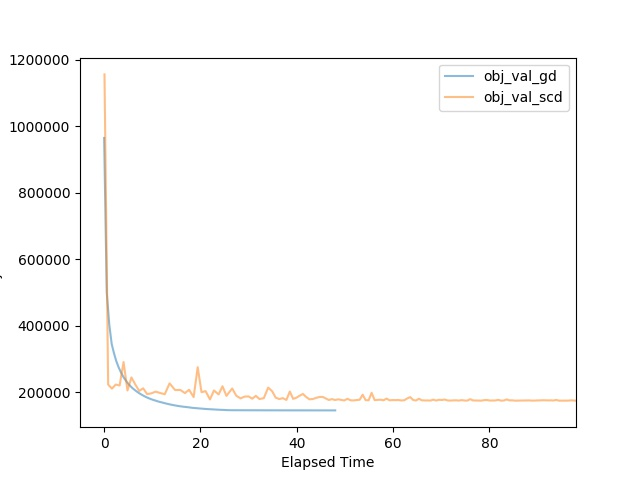
\includegraphics[width=0.6\columnwidth]{q4/plot.jpeg}%

\caption{Objective Value against wall clock time for Gradient Decent and Stochastic Coordinate Descent }
  
\label{fig:proto}%
\end{figure}
According to Wall Clock Time: \\
At the start SCD reduces the value faster but after initial fast reduction it becomes slower and GD reaches a better optimal value earlier.  
\newpage 
\subsection*{Part 6:} 
 
\begin{figure}[th]%
\centering

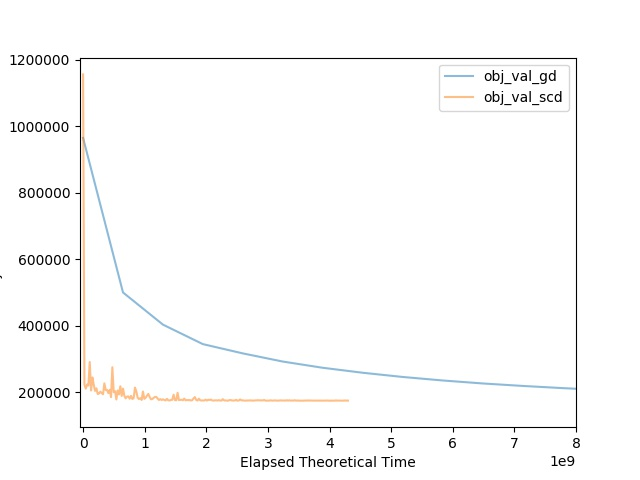
\includegraphics[width=0.6\columnwidth]{q4/theoretical.jpeg}%

\caption{Objective Value against theoretical time for Gradient Decent and Stochastic Coordinate Descent }
\label{fig:proto}%
\end{figure}
In theoretical time SCD is much much faster in converging ! I had to cut the graph along x-axis to even see the scd plot properly. This clearly shows how less computations SCD really takes. 

 
 
 
\end{mlsolution}
					
\end{document}